\documentclass[crop,tikz]{standalone}

\usepackage{makecell}

\definecolor{alizarin}{rgb}{0.82, 0.1, 0.26}
\definecolor{airforceblue}{rgb}{0.36, 0.54, 0.66}
\definecolor{apricot}{rgb}{0.98, 0.81, 0.69}
\definecolor{blush}{rgb}{0.87, 0.36, 0.51}
\definecolor{cadmiumgreen}{rgb}{0.0, 0.42, 0.24}
\definecolor{cambridgeblue}{rgb}{0.64, 0.76, 0.68}
\definecolor{celadon}{rgb}{0.67, 0.88, 0.69}
\definecolor{chestnut}{rgb}{0.8, 0.36, 0.36}
\definecolor{harvardcrimson}{rgb}{0.79, 0.0, 0.09}
\definecolor{darkseagreen}{rgb}{0.56, 0.74, 0.56}
\definecolor{aoenglish}{rgb}{0.0, 0.5, 0.0}
\definecolor{brightube}{rgb}{0.82, 0.62, 0.91}

\usetikzlibrary{positioning}
\usetikzlibrary{matrix}
\usetikzlibrary{fit}
\usetikzlibrary{calc,decorations.pathmorphing,patterns}

\newcommand{\vvector}[1]{\tikz{\draw[#1,step=1em,fill=#1!50] (0,0)  grid (1em,4em) rectangle (0, 0);}}
\newcommand{\hvector}[1]{\tikz{\draw[#1,step=1em,fill=#1!50] (0,0)  grid (4em,1em) rectangle (0, 0);}}
\newcommand{\vvectorSmall}[1]{\tikz{\draw[#1,step=.5em,fill=#1!50] (0,0)  grid (.5em,1.5em) rectangle (0, 0);}}

\newdimen\XCoord
\newdimen\YCoord
\newdimen\XXCoord
\newdimen\YYCoord

\newcommand{\outgoing}[2]{
  \path (#1); \pgfgetlastxy{\XCoord}{\YCoord};
  \path (#2); \pgfgetlastxy{\XXCoord}{\YYCoord};
  \draw[->, line width=1pt] (\XCoord, \YCoord) -- (\XCoord, \YYCoord);
}%
\newcommand{\incoming}[2]{
  \path (#1); \pgfgetlastxy{\XCoord}{\YCoord};
  \path (#2); \pgfgetlastxy{\XXCoord}{\YYCoord};
  \draw[->, line width=1pt] (\XCoord, \YYCoord) -- (\XCoord, \YCoord);
}%


%\newcommand{\selfattention}{couche d'auto-attention}
%\newcommand{\boxLabel}{couche d'encodage}
%\newcommand{\ff}{couche à propagation avant}
%\newcommand{\irepr}{\makecell{i-ème représentations \\ intermédiaires}}
%\newcommand{\irepr}{\makecell{(i+1)-ème représentations \\ intermédiaires}}


\newcommand{\selfattention}{self-attention layer}
\newcommand{\boxLabel}{encoder layer}
\newcommand{\ff}{feed-forward layer}
\newcommand{\irepr}{\makecell{$i$-th intermediate \\ representation}}
\newcommand{\iirepr}{\makecell{$(i+1)$-th intermediate \\ representation}}


\begin{document}

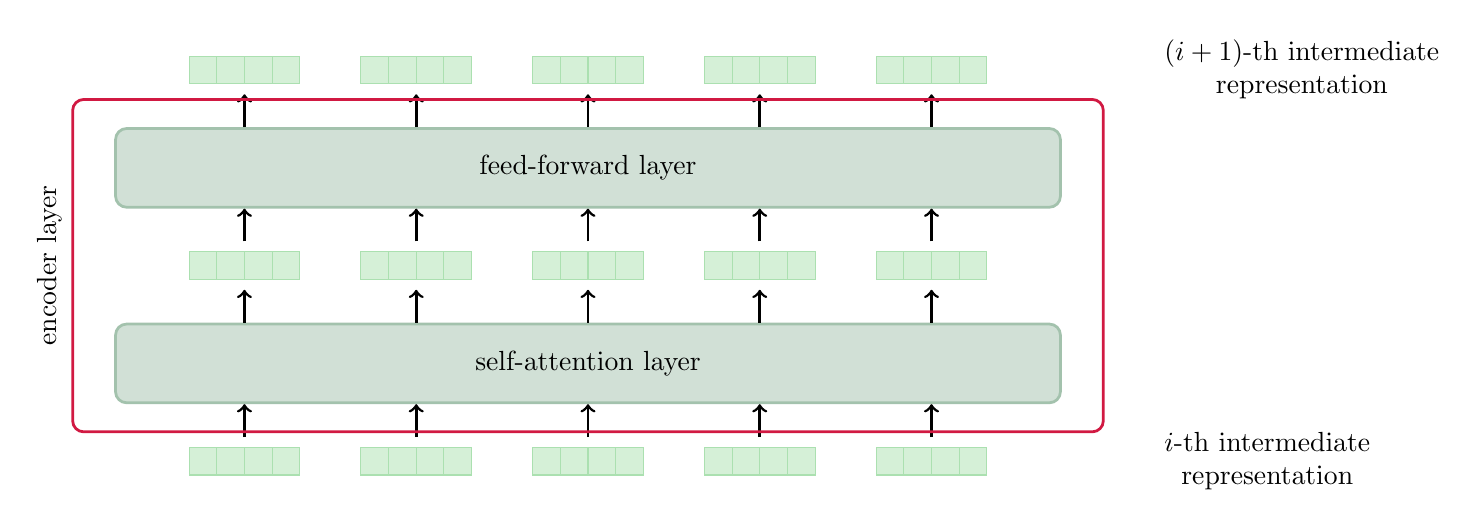
\begin{tikzpicture}[ampersand replacement=\&]
    \tikzset{node distance = .3cm and 2cm}
    
    \node[rounded corners, draw=cambridgeblue, fill=cambridgeblue!50, line width=1pt, minimum height=1cm, minimum width=12cm] (ff) {\ff};
    
    \matrix (M) [matrix of nodes,
    row sep=3em,
    column sep=1.5em,
    below=of ff,
    minimum width=2em,]
    { \hvector{celadon} \&
      \hvector{celadon} \&
      \hvector{celadon} \&
      \hvector{celadon} \&
      \hvector{celadon} \\
    };
    
    \node[rounded corners, draw=cambridgeblue, fill=cambridgeblue!50, line width=1pt, minimum height=1cm, minimum width=12cm, below=of M] (selfattention) {\selfattention};
    
    \outgoing{M-1-1.north}{ff.south}
    \outgoing{M-1-2.north}{ff.south}
    \outgoing{M-1-3.north}{ff.south}
    \outgoing{M-1-4.north}{ff.south}
    \outgoing{M-1-5.north}{ff.south}


    \incoming{M-1-1.south}{selfattention.north}
    \incoming{M-1-2.south}{selfattention.north}
    \incoming{M-1-3.south}{selfattention.north}
    \incoming{M-1-4.south}{selfattention.north}
    \incoming{M-1-5.south}{selfattention.north}
    
    \matrix (input) [matrix of nodes,
                     column sep=1.5em,
                     below=of selfattention,
                     minimum width=2em,]
    { \hvector{celadon} \&
      \hvector{celadon} \&
      \hvector{celadon} \&
      \hvector{celadon} \&
      \hvector{celadon} \\
    };

    \outgoing{input-1-1.north}{selfattention.south}
    \outgoing{input-1-2.north}{selfattention.south}
    \outgoing{input-1-3.north}{selfattention.south}
    \outgoing{input-1-4.north}{selfattention.south}
    \outgoing{input-1-5.north}{selfattention.south}

    \matrix (output) [matrix of nodes,
                     column sep=1.5em,
                     above=of ff,
                     minimum width=2em,]
    { \hvector{celadon} \&
      \hvector{celadon} \&
      \hvector{celadon} \&
      \hvector{celadon} \&
      \hvector{celadon} \\
    };

    \incoming{output-1-1.south}{ff.north}
    \incoming{output-1-2.south}{ff.north}
    \incoming{output-1-3.south}{ff.north}
    \incoming{output-1-4.south}{ff.north}
    \incoming{output-1-5.south}{ff.north}

    \node[draw=alizarin, rounded corners, line width=1pt, fit=(ff) (selfattention), inner xsep=1.5em, inner ysep=1em] (box) {};

    \node[rotate=90, above] at (box.west) {\boxLabel};
    
    \node [right=of input-1-5] {\irepr};
    \node [right=of output-1-5] {\iirepr};

\end{tikzpicture}

\end{document}